%%%%%%%%%%%%%%%%%%%%%%%%%%%%%%%%%%%%%%%%%%%%%%%%%%%%%%%%%%%%%%%%%%%%%%%%%%%%%%%%%%%%%%%%%%%%%%%%%%%
% Appendix -> Supplementary Tables and Figures of PHLOWER
% Author: Mingbo Cheng
%%%%%%%%%%%%%%%%%%%%%%%%%%%%%%%%%%%%%%%%%%%%%%%%%%%%%%%%%%%%%%%%%%%%%%%%%%%%%%%%%%%%%%%%%%%%%%%%%%%
\chapter{Appendix B: PHLOWER}
\label{chapter:appendixB}

\setstretch{1}

\graphicspath{{appendix/figs}}

\begin{figure}[!ht]
  \centering
  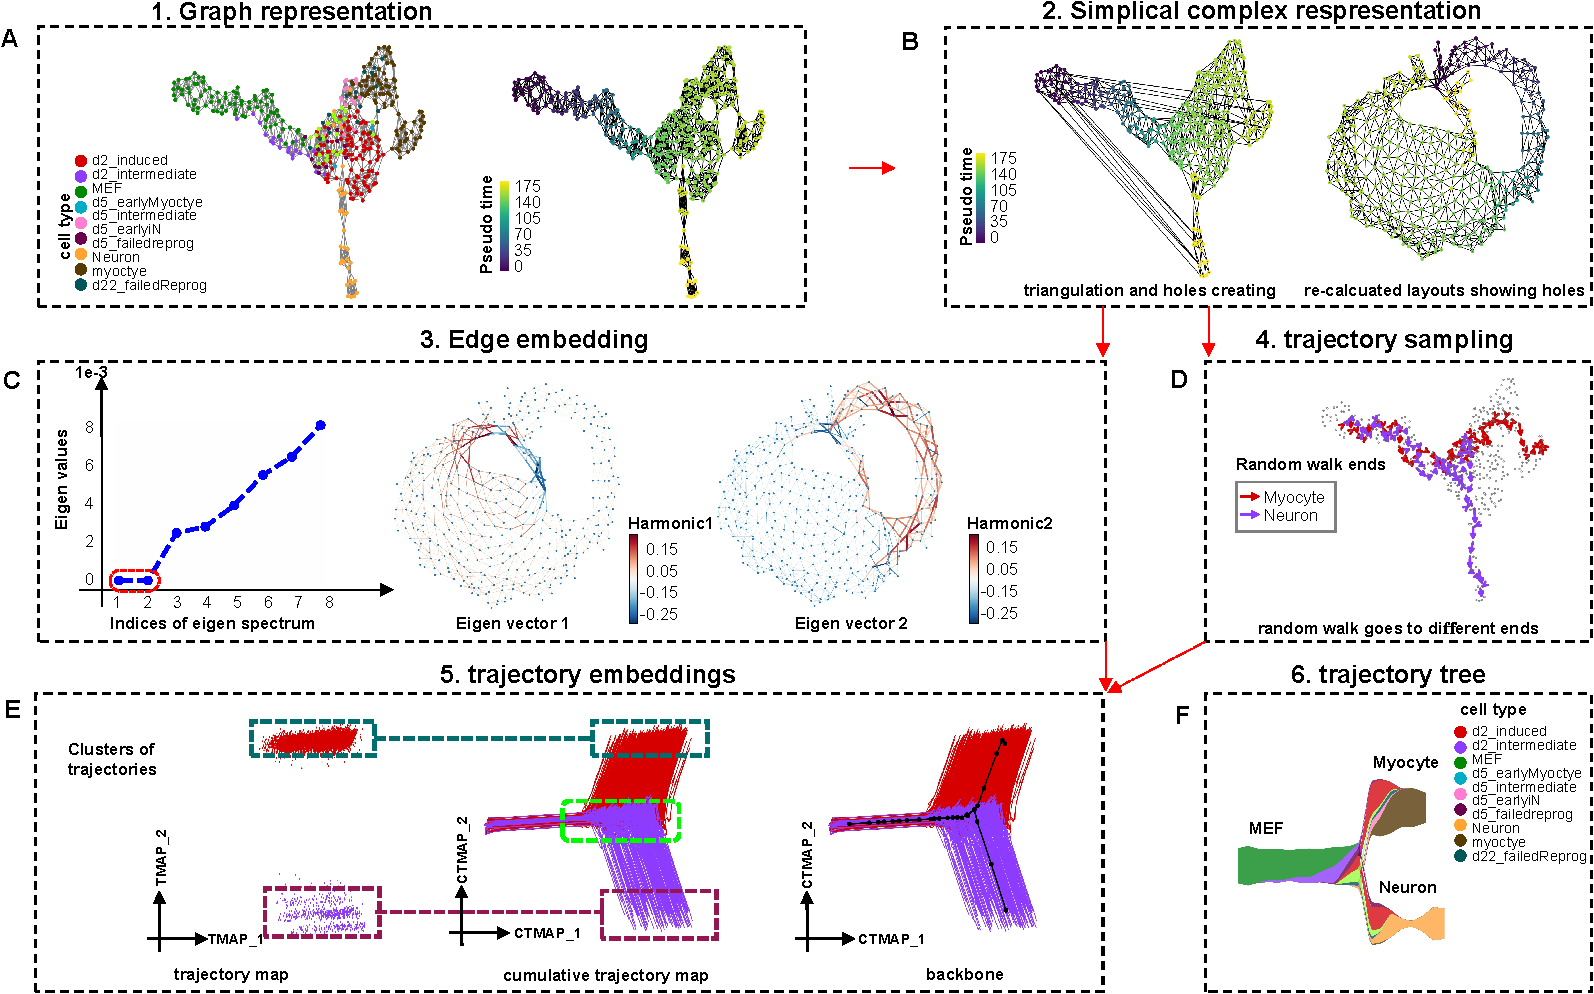
\includegraphics[width=0.95\textwidth]{Fib2Neuron_PHLOWER/fig}
  \vspace{0.1cm}
  \caption[Fibroblasts to Neurons dataset PHLOWER workflow.]{\textbf{Fibroblasts to Neurons dataset PHLOWER workflow}.}
  \label{supfig:fib2neuron-workflow}
\end{figure}


\begin{figure}[!ht]
  \centering
  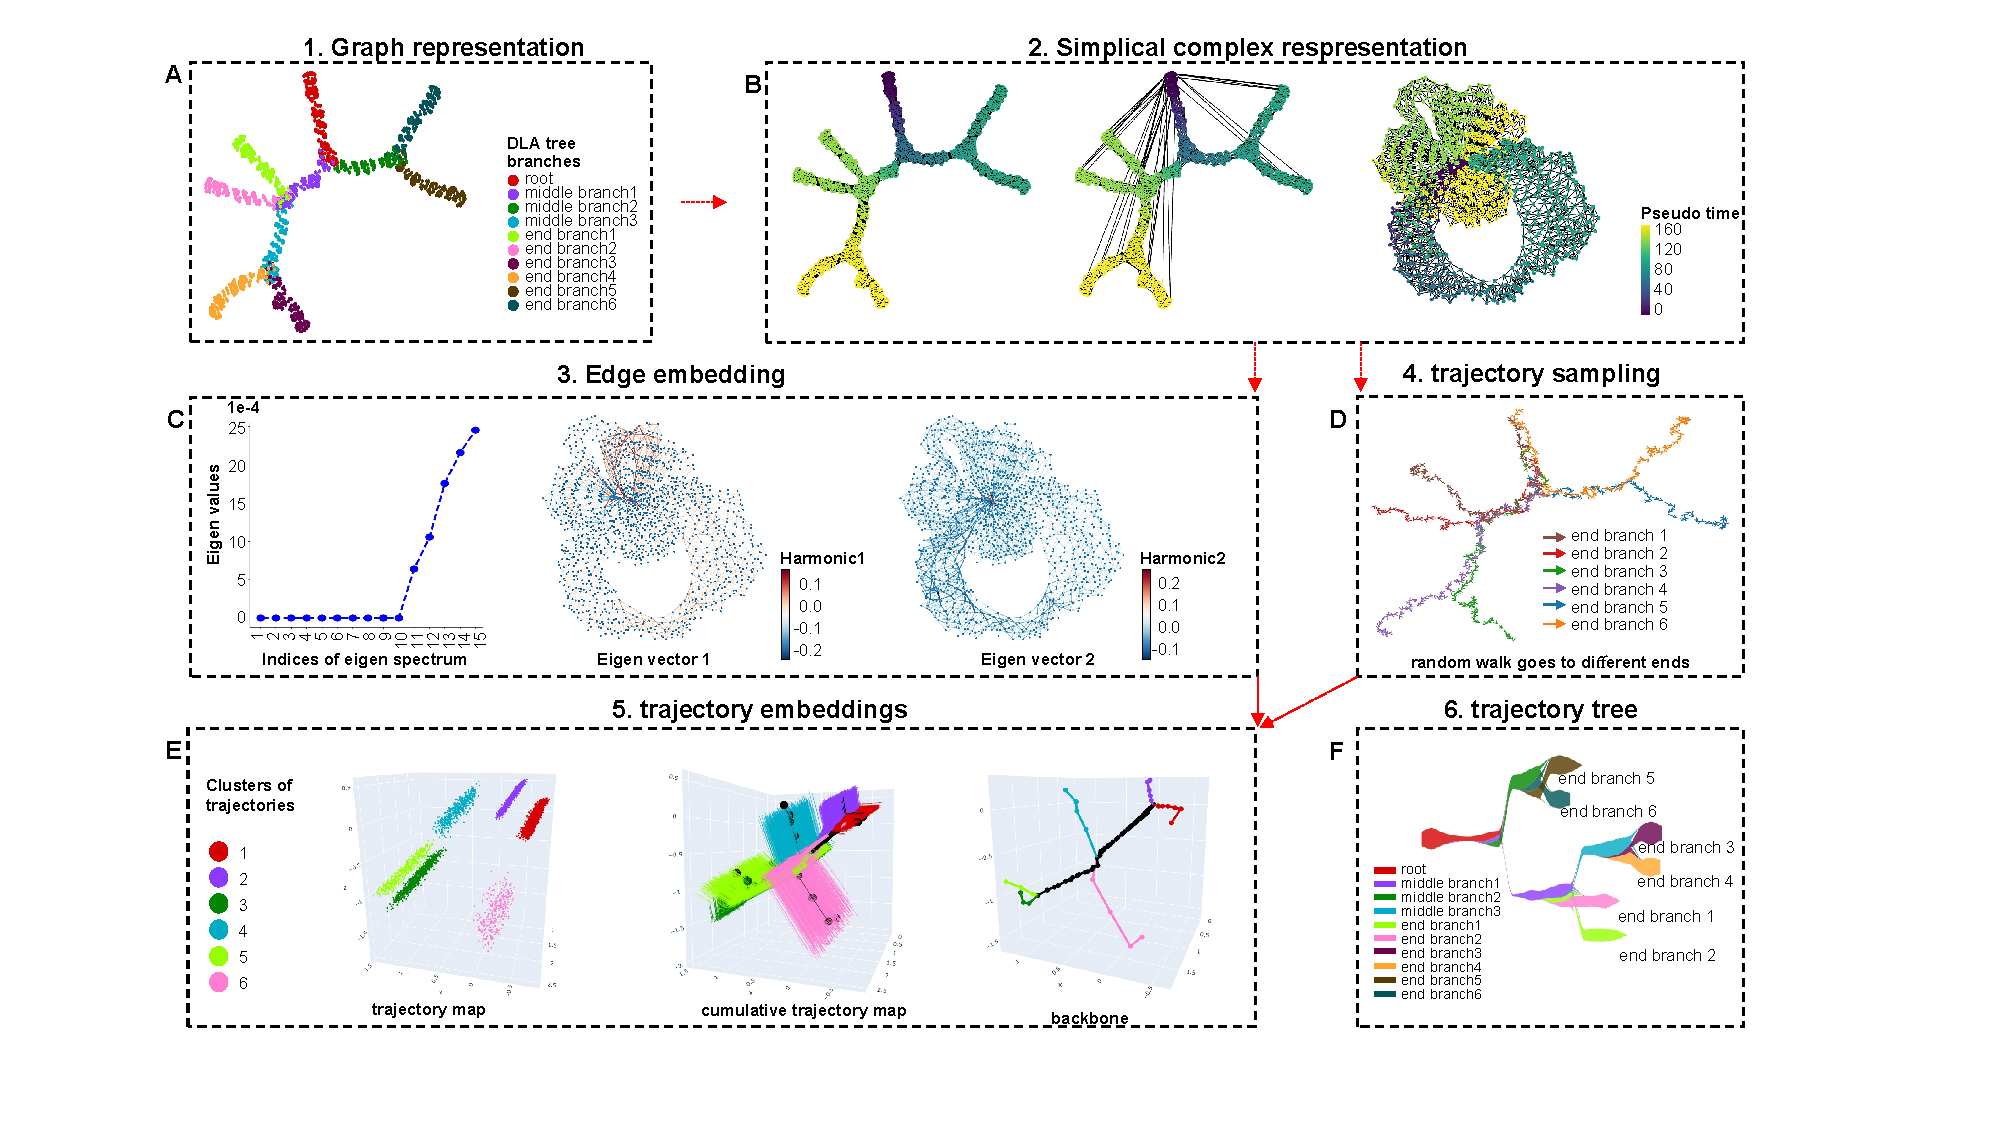
\includegraphics[width=0.95\textwidth]{DLA10_PHLOWER/fig}
  \vspace{0.1cm}
  \caption[Workflow for DLA simulated data.]{\textbf{Workflow for DLA simulated data}.}
  \label{supfig:dla10-workflow}
\end{figure}


\begin{figure}[!ht]
  \centering
  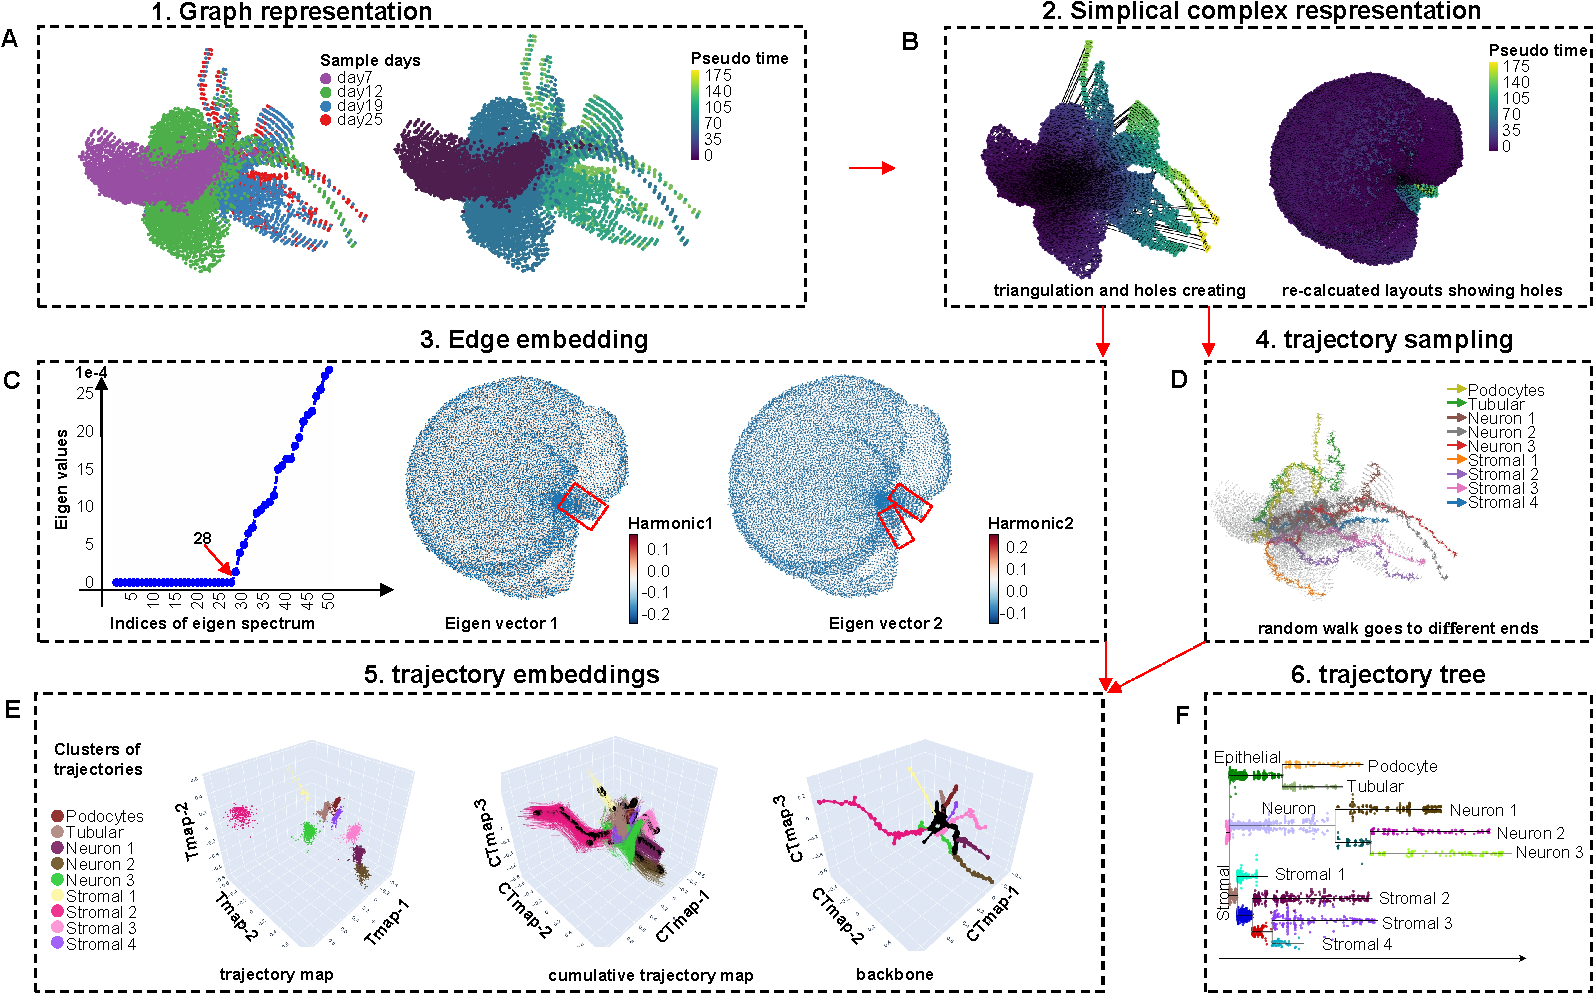
\includegraphics[width=0.95\textwidth]{kidney_PHLOWER//fig}
  \vspace{0.1cm}
  \caption[Kidney organoid PHLOWER workflow.]{\textbf{Kidney organoid PHLOWER workflow}.}
  \label{supfig:kidney-workflow}
\end{figure}







\begin{table}[!ht]
\centering
\caption[Friedman-Nemenyi test of TI's structure similarity]{\textbf{Friedman-Nemenyi test of TI's structure similarity.} Asterisks indicate P-values of $<0.05$(*), $<0.01$(**), $<0.001$(***), $<0.0001$(****) obtained via Friedman-Nemenyi test}
\begin{tabular}{rlllllllllll}
  \hline
 & \rotatebox{60}{phlower} &
   \rotatebox{60}{paga\_tree} &
   \rotatebox{60}{monocle3} &
   \rotatebox{60}{raceid\_stemid} &
   \rotatebox{60}{stream} &
   \rotatebox{60}{pcreode} & 
   \rotatebox{60}{tscan} &
   \rotatebox{60}{elpigraph} & 
   \rotatebox{60}{slingshot} &
   \rotatebox{60}{mst} &
   \rotatebox{60}{celltree\_vem} \\
  \hline
paga\_tree &  &  &  &  &  &  &  &  &  &  &  \\
  monocle3 &  &  &  &  &  &  &  &  &  &  &  \\
  raceid\_stemid &  &  &  &  &  &  &  &  &  &  &  \\
  stream &  &  &  &  &  &  &  &  &  &  &  \\
  pcreode & * &  &  &  &  &  &  &  &  &  &  \\
  tscan & * &  &  &  &  &  &  &  &  &  &  \\
  elpigraph & * &  &  &  &  &  &  &  &  &  &  \\
  slingshot & ** &  &  &  &  &  &  &  &  &  &  \\
  mst & **** & * & * &  &  &  &  &  &  &  &  \\
  celltree\_vem & **** & ** & * & * &  &  &  &  &  &  &  \\
  slice & **** & **** & **** & ** & ** & * &  &  &  &  &  \\
   \hline
\end{tabular}
\label{tab:him_asterisk}
\end{table}


\begin{table}[!ht]
\centering
\caption[Friedman-Nemenyi test of TI's cells location]{\textbf{Friedman-Nemenyi test of TI's cells location.} Asterisks indicate P-values of $<0.05$(*), $<0.01$(**), $<0.001$(***), $<0.0001$(****) obtained via Friedman-Nemenyi test}
\begin{tabular}{rlllllllllll}
  \hline
 & \rotatebox{60}{phlower} &
   \rotatebox{60}{paga\_tree} &
   \rotatebox{60}{monocle3} &
   \rotatebox{60}{raceid\_stemid} &
   \rotatebox{60}{stream} &
   \rotatebox{60}{pcreode} & 
   \rotatebox{60}{tscan} &
   \rotatebox{60}{elpigraph} & 
   \rotatebox{60}{slingshot} &
   \rotatebox{60}{mst} &
   \rotatebox{60}{celltree\_vem} \\
  \hline
raceid\_stemid &  &  &  &  &  &  &  &  &  &  &  \\
  tscan &  &  &  &  &  &  &  &  &  &  &  \\
  pcreode &  &  &  &  &  &  &  &  &  &  &  \\
  mst &  &  &  &  &  &  &  &  &  &  &  \\
  slingshot &  &  &  &  &  &  &  &  &  &  &  \\
  celltree\_vem &  &  &  &  &  &  &  &  &  &  &  \\
  paga\_tree & * &  &  &  &  &  &  &  &  &  &  \\
  elpigraph & * &  &  &  &  &  &  &  &  &  &  \\
  stream & **** &  &  &  &  &  &  &  &  &  &  \\
  slice & **** &  &  &  &  &  &  &  &  &  &  \\
  monocle3 & **** & * & * &  &  &  &  &  &  &  &  \\
   \hline
\end{tabular}
\label{tab:cordist_asterisk}
\end{table}


\begin{table}[!ht]
\centering
\caption[Friedman-Nemenyi test of TI's branches allocation]{\textbf{Friedman-Nemenyi test of TI's branches allocation.} Asterisks indicate P-values of $<0.05$(*), $<0.01$(**), $<0.001$(***), $<0.0001$(****) obtained via Friedman-Nemenyi test}
\begin{tabular}{rlllllllllll}
  \hline
 & \rotatebox{60}{phlower} &
   \rotatebox{60}{paga\_tree} &
   \rotatebox{60}{monocle3} &
   \rotatebox{60}{raceid\_stemid} &
   \rotatebox{60}{stream} &
   \rotatebox{60}{pcreode} & 
   \rotatebox{60}{tscan} &
   \rotatebox{60}{elpigraph} & 
   \rotatebox{60}{slingshot} &
   \rotatebox{60}{mst} &
   \rotatebox{60}{celltree\_vem} \\
  \hline
monocle3 &  &  &  &  &  &  &  &  &  &  &  \\
  paga\_tree &  &  &  &  &  &  &  &  &  &  &  \\
  raceid\_stemid &  &  &  &  &  &  &  &  &  &  &  \\
  slingshot &  &  &  &  &  &  &  &  &  &  &  \\
  tscan &  &  &  &  &  &  &  &  &  &  &  \\
  pcreode &  &  &  &  &  &  &  &  &  &  &  \\
  stream & * &  &  &  &  &  &  &  &  &  &  \\
  elpigraph & ** & * &  &  &  &  &  &  &  &  &  \\
  mst & ** & * &  &  &  &  &  &  &  &  &  \\
  celltree\_vem & **** & * &  &  &  &  &  &  &  &  &  \\
  slice & **** & **** & **** & ** & * & * &  &  &  &  &  \\
   \hline
\end{tabular}
\label{tab:f1branches_asterisk}
\end{table}


\begin{table}[!ht]
\centering
\caption[Friedman-Nemenyi test of TI's branch point allocation]{\textbf{Friedman-Nemenyi test of TI's branch point allocation.} Asterisks indicate P-values of $<0.05$(*), $<0.01$(**), $<0.001$(***), $<0.0001$(****) obtained via Friedman-Nemenyi test}
\begin{tabular}{rlllllllllll}
  \hline
& \rotatebox{60}{phlower} &
   \rotatebox{60}{paga\_tree} &
   \rotatebox{60}{monocle3} &
   \rotatebox{60}{raceid\_stemid} &
   \rotatebox{60}{stream} &
   \rotatebox{60}{pcreode} & 
   \rotatebox{60}{tscan} &
   \rotatebox{60}{elpigraph} & 
   \rotatebox{60}{slingshot} &
   \rotatebox{60}{mst} &
   \rotatebox{60}{celltree\_vem} \\
  \hline
raceid\_stemid &  &  &  &  &  &  &  &  &  &  &  \\
  monocle3 &  &  &  &  &  &  &  &  &  &  &  \\
  paga\_tree &  &  &  &  &  &  &  &  &  &  &  \\
  tscan &  &  &  &  &  &  &  &  &  &  &  \\
  slingshot &  &  &  &  &  &  &  &  &  &  &  \\
  pcreode &  &  &  &  &  &  &  &  &  &  &  \\
  stream &  &  &  &  &  &  &  &  &  &  &  \\
  mst & * &  &  &  &  &  &  &  &  &  &  \\
  elpigraph & ** &  &  &  &  &  &  &  &  &  &  \\
  celltree\_vem & ** &  &  &  &  &  &  &  &  &  &  \\
  slice & **** & **** & **** & ** & ** & ** &  &  &  &  &  \\
   \hline
\end{tabular}
\label{tab:f1milestone_asterisk}
\end{table}
